 \documentclass{article}

\usepackage{geometry}
\usepackage{graphicx}
\usepackage{amsmath}

\title{Interfacing HD44780U LCD display and MCS-51 based microcontroller in EDISM simulator -- an EMISY laboratory}
\author{Maciej Marcinkiewicz (300171)}
\date{29th April 2021}

\newgeometry{lmargin=3.2cm, rmargin=3.2cm, bmargin=2.5cm}

\begin{document}

\maketitle

\section{Introduction}
\subsection{Brief description}
Laboratory's main purpose was to learn the basiscs of MCS-51 (Intel 8051) assembly
programming and to learn the way of proper dealing with 2x16 Hitachi HD44780U based displays.
The task was to use 8051 microcontroller to print some characters to the LCD.

\subsection{Schematic}
\begin{figure}[h!] %possible: b, t, h, p and override (!)
    \centering
        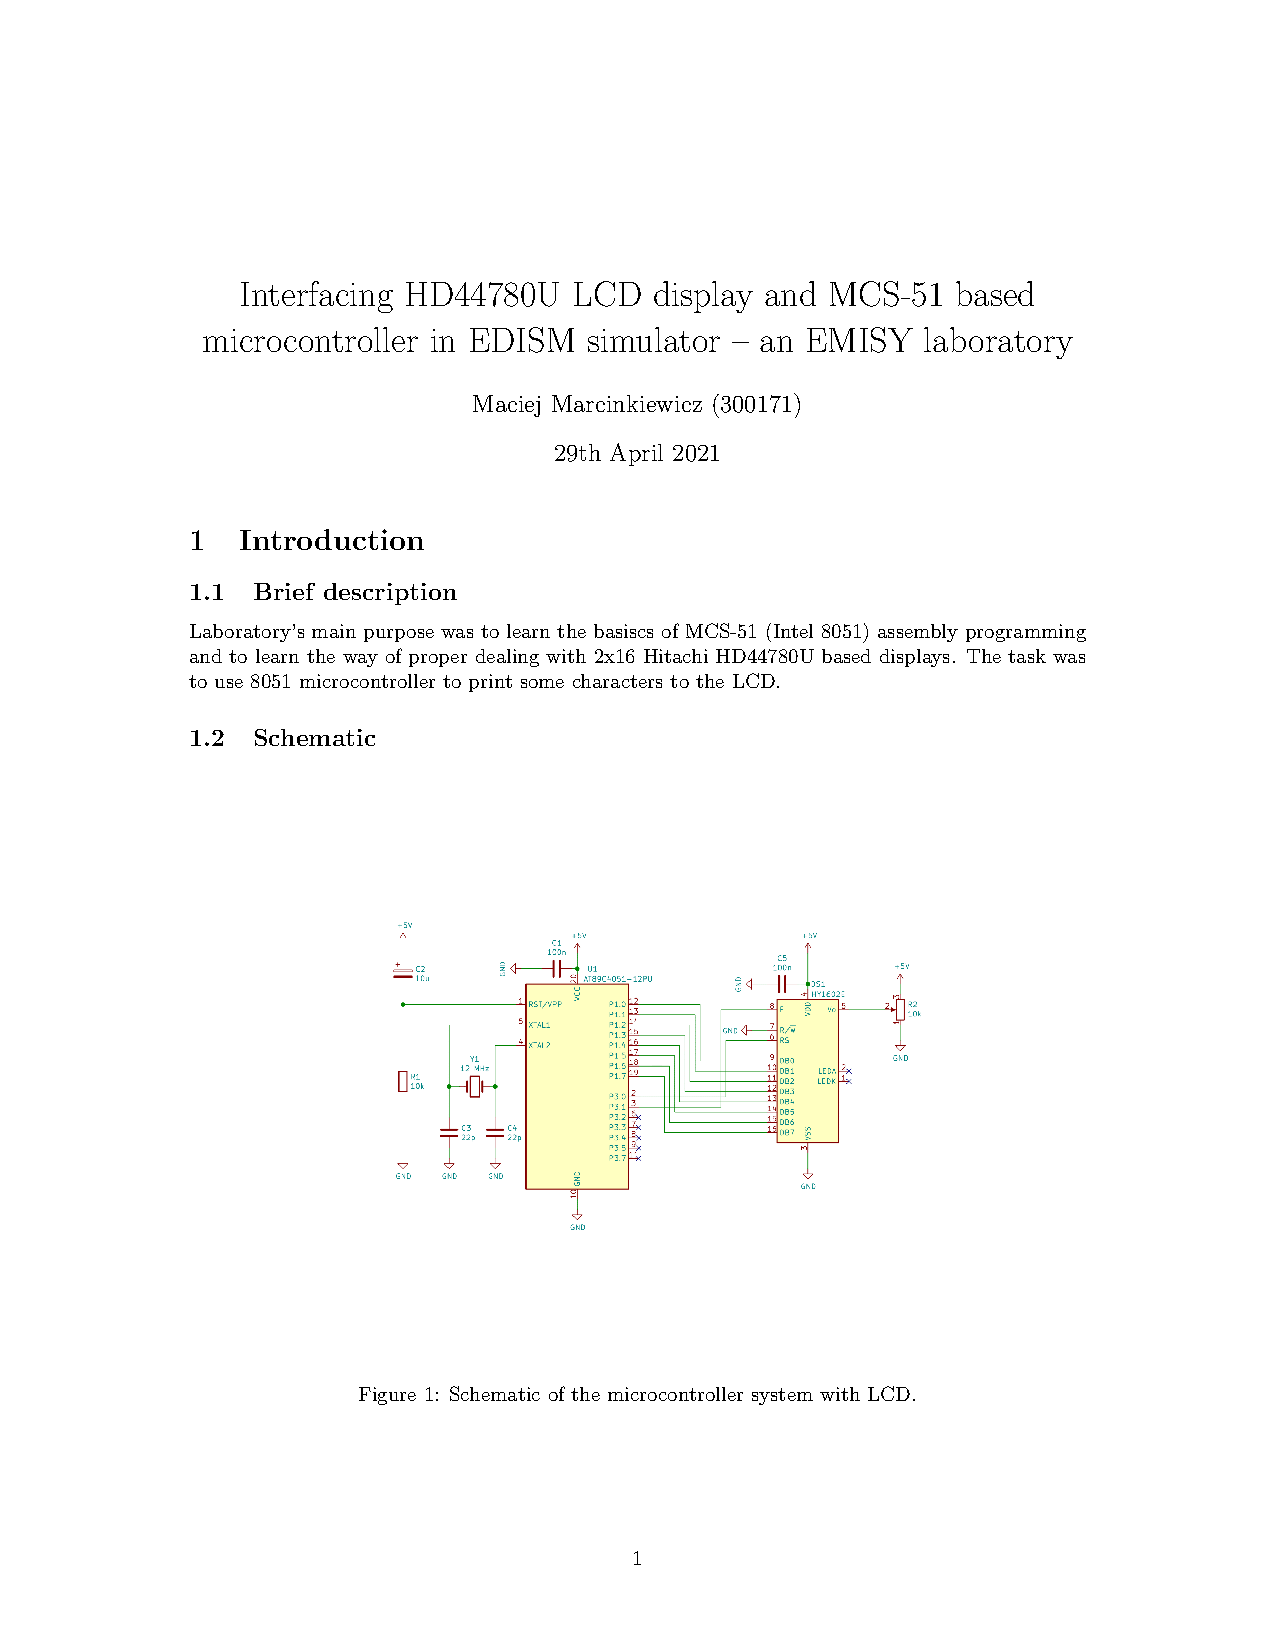
\includegraphics[width=0.9\linewidth]{schematics/lab1.png}
    \caption{Schematic of the microcontroller system with LCD.}
\end{figure}

\subsection{Hardware description}
Microcontroller (Atmel's AT89C4051) is connected to 5 V source and is equipped with 12 MHz clock and 
simple resetting circuit. LCD (HY1602E) is also connected to 5 V source. Its data bus is connected
to P1 GPIO port of the microcontroller unit. RS and E pins are connected to the P3.0 and P3.1,
respectively. LEDA and LEDK pins are not used. R/W pin is grounded, which corresponds to
permanent write (W) mode. Contrast pin V$_0$ is connected to the standard in this case 10 k$\Omega$ potentiometer.

\section{Task 1}
\subsection{Code description}
\subsubsection{8-bit mode}
Program starts with constants definition. In order to make the code more readable,
pins has been assigned to mnemonic names. Then the main routine starts with display
initialization. Assigning immiediate value to the register and decrementing it makes
a simple loop which is required for delay. In the beginning microcontroller has to wait
for display at least 30 miliseconds (in order to get proper voltage on display).
Program calls \texttt{long\textunderscore delay} subroutine 20 times in order to wait this amount of time.

\texttt{long\textunderscore delay} decrements number 256 to zero three times. It gives
appoximately 1.53 ms (even more than this). This number is not coincidence -- such delay
will be used later when several characters will be printed on display.

After 30 ms of delay data bus is filled with value responsible for function set. 
Display has to be set to two line mode. Then command is being sent by \texttt{send\textunderscore command}
subroutine. It clears RS pin as command is being sent, not data about character. In the end
it sets and then clears E pin. It is a signal for display to get data from data bus. The last
step is a short delay before the next command. \texttt{short\textunderscore delay} subroutine
is even simpler than \texttt{long\textunderscore delay}. It only decrements to zero value of 18.
It results in delay of more than 39 $\mu$s which is necessary after executing each display's command.

The next command is responsible for turning on the display and showing cursor. It is executed
in the same manner as function set. The last step in initialization process is entering
set mode. It is set to increment mode, so characters are appearing one after the other.

When initialization is finished, program is writing letter M into display's DDRAM (in the first postiton of the first line).
Letter's code is written to the data bus and \texttt{send\textunderscore data} is called.
It works almost in the same way as \texttt{send\textunderscore command}, the only difference is that
it sets R/S pin to turn on writing mode. Code is finished with an infinite loop.


\end{document}